\documentclass{article}

\usepackage{amsmath}
\usepackage{amssymb}
\usepackage{enumerate}
\usepackage{graphicx}
\usepackage{subcaption}
\usepackage{interval}

\intervalconfig{soft open fences}

\newcommand{\solution}[1]{%
\ifsolutions%
    \textbf{Solution: } #1
\fi
}

\title{PAMO Shortlist}
\author{}
\date{2018}

\begin{document}

\maketitle

\section{Algebra}
\begin{enumerate}

\item Find all functions $f : \mathbb{Z} \to \mathbb{Z}$ such that ${(f(x + y))}^2 = f(x^2) + f(y^2)$ for all $x, y \in \mathbb{Z}$.

\solution{Let $x = y = 0$. We find that ${(f(0))}^2 = 2f(0)$, and so either $f(0) = 0$ or $f(0) = 2$.

If $f(0) = 0$, then letting $y = 0$ in the functional equation gives us that ${(f(x))}^2 = f(x^2)$, and so the functional equation becomes ${(f(x + y))}^2 = {f(x)}^2 + {f(y)}^2$. We see that the function $x \mapsto {(f(x))}^2$ satisfies the Cauchy functional equation, and so ${(f(x))}^2 = x{(f(1))}^2$ for all $x$. This implies that $x{(f(1))}^2$ is always non-negative, which implies that $f(1) = 0$, giving us that ${(f(x))}^2 = 0$ for all $x$, and so $f(x) = 0$ for all $x$.

On the other hand, if $f(0) = 2$, then letting $y = 0$ in the functional equation gives us that ${(f(x))}^2 = f(x^2) + 2$. The functional equation thus becomes ${(f(x + y))}^2  = {(f(x))}^2 + {(f(y))}^2 - 4$. We see that the function $x \mapsto {(f(x))}^2 - 4$ satisfies the Cauchy functional equation, and so we obtain that ${(f(x))}^2 - 4 = x({(f(1))}^2 - 4)$ for all $x$. As before, since the LHS is bounded below by $-4$, the RHS is also bounded below, and so must be identically $0$. We thus have that ${(f(x))}^2 = 4$ for all $x$.

It follows that for each $x$, we have that $f(x) = 2$ or $f(x) = -2$. Thus for any $x$ and $y$, we have that
\[
    f(x^2) + f(y^2) = {(f(x + y))}^2 = 4,
\]
which implies that $f(x^2) = f(y^2) = 2$. It is easy to check that any function $f$ such that $f(x) = 2$ or $f(x) = -2$ for all $x$, and such that $f(x) = 2$ if $x$ is a square satisfies the functional equation.}

\item Find a non-zero polynomial $f(x, y)$ such that $f(\lfloor 3t \rfloor, \lfloor 5t \rfloor) = 0$ for any $t \in \mathbb{R}$.

\solution{Let $x = \lfloor 3t \rfloor$ and $y = \lfloor 5t \rfloor$, where $t \in \mathbb{R}$ and define $f(x, y) = 5x - 3y$. We claim that $f(x, y) = 0, \pm 1, \pm 2, -3, -4$. For any integer $k$, we have $5 \lfloor 3(t + k) \rfloor - 3 \lfloor 5(t + k) \rfloor = 5(\lfloor 3t \rfloor + 3k) - 3(\lfloor 5t \rfloor + 5k) = 5 \lfloor 3t \rfloor - 3 \lfloor 5t \rfloor$. So $f(\lfloor 3t \rfloor, \lfloor 5t \rfloor) = 5 \lfloor 3t \rfloor - 3 \lfloor 5t \rfloor$ is periodic function with period $1$. It suffices to consider $t \in \interval[open right]{0}{1}$. We now partition $\interval[open right]{0}{1}$ as follows: $\interval[open right]{0}{1} = [0, \frac{1}{5}) \cup [\frac{1}{5}, \frac{1}{3}) \cup [\frac{1}{3}, \frac{2}{5}) \cup [\frac{2}{5}, \frac{3}{5}) \cup [\frac{3}{5}, \frac{2}{3}) \cup [\frac{2}{3}, \frac{4}{5}) \cup [\frac{4}{5}, 1)$. So,
\[
    f(x, y) = 5x - 3y = 5 \lfloor 3t \rfloor - 3 \lfloor 5t \rfloor =
    \begin{cases}
        0,      & t \in \interval[open right]{0}{\frac{1}{5}}, \\
        -3,     & t \in \interval[open right]{\frac{1}{5}}{\frac{1}{3}}, \\
        2,      & t \in \interval[open right]{\frac{1}{3}}{\frac{2}{5}}, \\
        -1,     & t \in \interval[open right]{\frac{2}{5}}{\frac{3}{5}}, \\
        -4,     & t \in \interval[open right]{\frac{3}{5}}{\frac{2}{3}}, \\
        1,      & t \in \interval[open right]{\frac{2}{3}}{\frac{4}{5}}, \\
        -2,     & t \in \interval[open right]{\frac{4}{5}}{1}.
    \end{cases}
\]

So $f(x, y) = (5x - 3y)({(5x - 3y)}^2 - 1)({(5x - 3y)}^2 - 4)(5x - 3y + 3)(5x - 3y + 4)$.}

\item Akello divides a square up into finitely many white and red rectangles, each (rectangle) with sides parallel to the sides of the paren square. Within each white rectangle, she writes down the value of its width divided by its height, while within each red rectangle, she writes down the value of its height divided by its width. Finally, she calculates $x$, the sum of these numbers. If the total are of the white rectangles equals the total area of the red rectangles, what is the least possible value of $x$ she can get?

\solution{Let $a_i$ and $b_i$ denote the width and height of each white rectangle, and $c_i$ and $d_i$ denote the width and height of each red rectangle. Also, let $\ell$ denote the side length of the original square. We claim that, either $\sum a_i \geq \ell$ or $\sum d_i \geq l$. We prove this as follows: \textit{suppose there exists a horizontal line across the square that is covered entirely with white rectangles. Then, the total width of these rectangles is at least $\ell$, and the claim is proven. Otherwise, there is a red rectangle intersecting every horizontal line, and hence the total height of these rectangles is at least $\ell$.} Without loss of generality, assume $\sum a_i \geq \ell$. By the Cauchy-Schwarz inequality, $\sum \frac{a_i}{b_i} \sum{a_i b_i} \geq {(\sum a_i)}^2 \geq \ell^2$. The total area of the white rectangles is half of that of the square, so $\sum a_i b_i = \frac{1}{2} \ell^2$, and so $\sum \frac{a_i}{b_i} \geq 2$. Furthermore, each $x_i \leq \ell$, so $\sum{d_i}{c_i} \geq \frac{1}{\ell} \sum d_i \geq \frac{1}{\ell^2} \sum c_i d_i = \frac{1}{2}$. Therefore, $x$ is at least $2.5$. Conversely, $x = 2.5$ can be achieved by making the top half of the square one colour, and the bottom half the other colour.}

\item Let $a, b, c$ and $d$ be non-zero pairwise different real numbers such that 
\[
    \frac{a}{b} + \frac{b}{c} + \frac{c}{d} + \frac{d}{a} = 4 \text{ and } ac = bd.
\]

Show that
\[
    \frac{a}{c} + \frac{b}{d} + \frac{c}{a} + \frac{d}{b} \leq -12
\]
and that $-12$ is the maximum.

\solution{Set $A = \frac{a}{c} + \frac{b}{d} + \frac{c}{a} + \frac{d}{b}$. As $ac = bd$, we have
\[
    A = \frac{a^2 + b^2 + c^2 + d^2}{ac} = \frac{{(a + c)}^2 + {(b + d)}^2 - 2ac - 2bd}{ac} = \frac{{(a + c)}^2 + {(b + d)}^2}{ac} - 4.
\]

Using $AGM$, we get
\[
    {(a + c)}^2 + {(b + d)}^2 \geq 2 |a + c| |b + d|. (\star)
\]

From $\frac{a}{b} + \frac{b}{c} + \frac{c}{d} + \frac{d}{a} = 4$ and $ac = bd$, we get
\[
    4 = \frac{a}{b} + \frac{b}{c} + \frac{c}{d} + \frac{d}{a} = \frac{ad + ba + bc + bd}{ac} = \frac{(a + c)(b + d)}{ac},
\]
so
\[
    (a + c)(b + d) = 4ac. (\star \star)
\]

Assume that $ac = bd > 0$. As $a \neq c$, we get through AGM $|a + c| > 2 \sqrt{ac}$, and similarly $|b + d| > 2 \sqrt{ac}$.

Since $ac > 0$, we have $(a + c)(b + d) > 0$, and so
\[
    (a + c)(b + d) = |a + c| |b + d| > 2 \sqrt{ac} \cdot 2 \sqrt{ac} = 4ac,
\]
in contradiction with $(\star \star)$.

Consequently, the real numbers $a, b, c$ and $d$ pairwise different satisfying $\frac{a}{b} + \frac{b}{c} + \frac{c}{d} + \frac{d}{a} = 4$ and $ac = bd$ are such that $ac = bd < 0$. In this case the relation $(\star)$ implies
\[
    \frac{{(a + c)}^2 + {(b + d)}^2}{ac} \leq \frac{2 |a + c| |b + d|}{ac} = - \frac{2(a + c)(b + d)}{ac} = -8.
\]

Hence $A \leq -12$. We can check that the value $-12$ is attained for example with $a = 1, b = -1, c = 3 + 2 \sqrt{2}$ and $d = -3 - 2 \sqrt{2}$.}

\item Let $g : \mathbb{N} \to \mathbb{N}$ be a function satisfying:
\begin{enumerate}
    \item $g(xy) = g(x)g(y), \forall x, y \in \mathbb{N}$,
    \item $g(g(x)) = x, \forall x \in \mathbb{N}$,
    \item $g(x) \neq x$ for $2 \leq x \leq 2018$.
\end{enumerate}

Find the minimum value of $g(2)$.

\solution{(Ans: $g(2) \geq 1013$).

Set $y = 1$ in i., then $g(1) = 1$.

We will show that $g$ maps primes to primes. Suppose that $p$ is a prime and $g(p)$ is not prime, then we can write $g(p) = xy$ for some $x \neq 1$, $y \neq 1$, so $p = g(g(p)) = g(xy) = g(x) g(y)$. Therefore WLOG $g(x) = 1$ since $p$ is prime, but $x = g(g(x)) = g(1) = 1$ which yields a contradiction, thus $g(p)$ is prime.

Let $n \in \mathbb{N}$. Then $n$ has prime factorization, say $n = p_1^{\alpha_1} p_2^{\alpha_2} \dots p_k^{\alpha_k}$. Have $m = g(p_1^{\alpha_1} p_2^{\alpha_2} \dots p_k^{\alpha_k}) = {g(p_1)}^{\alpha_1} {g(p_2)}^{\alpha_2} \dots {g(p_k)}^{\alpha_k} = q_1^{\alpha_1} q_2^{\alpha_2} \dots q_k^{\alpha_k}$ by extension of i., where $q_i = f(p_i)$ are primes. Note that if $x = tg(t)$, $t \in \mathbb{N}$, then $g(x) = g(tg(t)) = g(t) g(g(t)) = g(t) t = x$. For $t > 1$, have $x > 1$, so by iii. $x \geq 2019$ to $tg(t) \geq 2019$. In particular, must have $g(2) \geq 1010$ but $g(2)$ is prime, so $g(2) \geq 1013$.

Next to show $g(2) = 1013$ is possible, observe that for all $2 \leq x \leq 2018$, $x$ is either a power of two in which case $g(2^n) = {g(2)}^n \neq 2^n$, or $x = 1013$, and again $g(1013) \neq 1013$, or $x$ has a prime divisor $p < 2018$, $p \neq 2, 1013$ so may choose $q > 2018$ and set $g(p) = q$ (if $g(p)$ has not been set before) then $q \mid g(x)$ and hence $x \leq 2018 < q \leq g(x)$. For any other prime $r$ not involved in the above procedure, may take $g(r) = r$. Finally, since $g$ is determined by primes we get a valid function $g$ with $g(2) = 1013$.}

\item Let $a, b, c$ be positive real numbers such that $a^3 + b^3 + c^3 = 5abc$.

Show that
\[
    \left( \frac{a + b}{c} \right) \left( \frac{b + c}{a} \right) \left( \frac{c + a}{b} \right) \geq 9.
\]

\solution{First we shall show that $a + b \geq c$. Let $c = t(a + b)$ then $a^3 + b^3 + t^3 (a^3 + b^3 + 3ab(a + b)) = 5tab(a + b)$, so $\frac{5t - 3t^3}{1 + t^3} = \frac{a^3 + b^3}{ab(a + b)} \geq 1$. Hence $(1 - t)(4t^2 + 4t - 1) \geq 0$.

Suppose $t > 1$ then $0 \geq 4t^2 + 4t - 1 > 7$. Therefore $1 \geq t$ and $a + b \geq t(a + b) = c$.

In a similar way we get $a + b - c \geq 0$, $b + c - a \geq 0$, $c + a - b \geq 0$. Multiply the three inequalities yields $a^2 (b + c) + b^2 (c + a) + c^2 ( a + b) \geq a^3 + b^3 + c^3 + 2abc = 7abc$. Thus $(a + b) (b + c) (c + a) = a^2 (b + c) + b^2 (c + a) + c^2 (a + b) + 2abc \geq 9abc$.

\textbf{Note:} Alternatively to get $a + b \geq c$ one may set $2x = b + c - a$, $2y = c + a - b$ and $2z = a + b - c$ to get $a = y + z$, $b = z + x$ and $c = x + y$. WLOG $a \geq b \geq c > 0$ so $y, z > 0$. Suppose $x < 0$, then $a^3 + b^3 + c^3 = 5abc$ becomes
\begin{align*}
    -xyz & = & (x + y + z)(x^2 + y^2 + z^2 - 2xy - 2yz - 2zx) \\
         & = & (x + y + z)({(y + z - x)}^2 - 4yz) \\
         & \geq & (x + y + z)({(y + z - x)}^2 - {(y + z)}^2) \\
         & \geq & (x + y + z)(-x)(2y + 2z - x) > z(-x)(2y).
\end{align*}

This yields a contradiction so $x, y, z \geq 0$.}

\item Let $f(n) = n + \lfloor \sqrt{n} \rfloor$. Prove that for every positive integer $m$, the integer sequence $m, f(m), f(f(m)), \dots$ contains at least one square of an integer.

\solution{Let the $m$'s be of the form $m = k^2 + j$, where $0 \leq j \leq 2k$. Split them into two sets, the set $A$ of all the $m$ with excess $j$, where $0 \leq j \leq k$ and the set $B$ with all those $m$'s with excess $j$, where$k < j < 2k + 1$. Then $\lfloor \sqrt{m} \rfloor = k$ since $k^2 \leq m \leq k^2 + 2k < k^2 + 2k + 1 = {(k + 1)}^2$. If $j = 0$, we have nothing to prove.

Assume that $m \in B$. As $\lfloor \sqrt{m} \rfloor = k$, we have $f(m) = m + \lfloor \sqrt{m} \rfloor = (k^2 + j) + k = {(k + 1)}^2 + j - k - 1$ with $0 \leq j - k - 1 \leq k  - 1 < k + 1$. So either $f(m)$ is a square or $f(m) \in A$. 
We consider the case where $m \in A$. So $f(m) = m + \lfloor \sqrt{m} \rfloor = m + k$, and $\lfloor \sqrt{m + k} \rfloor = k$ since $m + k = k^2 + j + k \leq k^2 + 2k < {(k + 1)}^2$. So $f(f(m)) = f(m + k) = m + k + \lfloor \sqrt{m + k} \rfloor = m + 2k = k^2 + j + 2k = {(k + 1)}^2 + j - 1$. So $f(f(m))$ is either a square or $f(f(m)) \in A$ with an excess $j - 1$ less than the excess $j$ of $m$. At each iteration, the excess will reduce and eventually it will hit $0$, whence we reach a square.}

\end{enumerate}

\section{Number Theory}
\begin{enumerate}

\item Does there exist positive integers $a, b, c$ such that $4(ab - a - c^2) = b$.

\solution{Suppose that such trio exists, so $4ab - 4a - b = 4c^2$, or equivalently, $(4a - 1)(b - 1) = 4c^2 + 1$. The integer $4a - 1$ has at least one prime divisor, say $q$, that is of the form $4k + 3$. Then $4c^2 \equiv -1 \pmod q$. However, by Fermat's theorem we have
\[
    1 \equiv {(2c)}^{q - 1} \equiv {(4c^2)}^{\frac{q-1}{2}} \equiv {(-1)}^{\frac{q-1}{2}} \pmod q,
\]
which is impossible since $\frac{q-1}{2} = 2k + 1$ is odd.}

\item A positive integer is called special if its digits can be arranged to form an integer divisible by $4$. How many of the integers from $1$ to $2018$ are special?

\solution{We characterise the integers which are not special. Recall that a natural number $n$ is divisible by $4$ if and only if the number formed by the last two digits of $n$ is divisible by $4$.

Suppose that $n$ is not special. First we consider the case where all of the digits of $n$ are even. If $n$ contains a digit, say $a$, which is divisible by $4$, then if $b$ is any other digit of $n$, we know that $10b + a \equiv a \equiv 0 \pmod 4$, and so the digits of $n$ can be rearranged to form a number divisible by $4$. (i.e. The one that ends in $ba$.) We see that there are no non-special numbers all of whose digits are even and which contain a $0, 4$, or $8$. (If $n$ does not contain another digit other than $a$, then $n$ itself is equal to $0$, $4$, or $8$, and so is special.)

Thus if $n$ contains only even digits, then $n$ consists only of the digits $2$ and $6$. Conversely, since none of $22$, $26$, $62$, and $66$ are divisible by $4$, we see that any natural number containing only the digits $2$ and $6$ is not special. It follows that the number of $m$ digit numbers which are not special and which contain only even digits is equal to $2^m$.

We now consider the case where $m$ contains an odd digit. Let this odd digit be $a$. Note that $10a \equiv 2 \pmod 4$, and so if $n$ contains a $2$ or a $6$, then the digits of $n$ can be rearranged to end in $a2$ or $a6$ both of which are divisible by $4$, and so $n$ would be special. We see that if $n$ is not special, then the only even digits which $n$ can contain are $0, 4$, and $8$.

Now suppose that $n$ contains two even digits. Then the digits of $n$ can be rearranged to form the number ending in those two digits. This number is divisible by $4$, and so $n$ is special. It follows that if $n$ is not special, then $n$ contains either only odd digits, or exactly one even digit which has to be a $0, 4$, or $8$. Conversely, we see that any such number is not special.

The number of $m$ digit numbers containing only odd digits is equal to $5^m$. The number of $m$ digit numbers containing exactly one $0, 4$, or $8$ and having the rest of its digits odd is equal to $2 \cdot 5^{m-1} + 3(m - 1) \cdot 5^{m - 1}$. This is because if the number starts with $0, 4$, or $8$, then it starts with a $4$, or $8$, and so there are $2$ options for the first digit, and $5$ options for each of the remaining digits. Otherwise, there are $(m - 1)$ options for which digit is equal to $0, 4$, or $8$, and $3$ options for what that digit is equal to. There are then again $5$ options for each of the remaining digits. We also note that this formula requires $m > 1$, since a one-digit number can not contain a $0, 4$ or $8$, and also contain an odd digit.

For $m > 1$, we thus have that there are $2^m + 5^m + 2 \cdot 5^{m-1} + 3(m-1) \cdot 5^{m-1}$ non-special numbers.

Using the above, we see that there are $7$ one-digit non-special numbers, $54$ two-digit non-special numbers, and $333$ three-digit non-special numbers. This gives a total of $394$ non-special numbers below $1000$.

We now consider the non-special numbers $n$ such that $1000 \leq n < 2000$. We note that these all start with a $1$, and so are a non-special number containing an odd digit. As before, we see that the remaining digits are either all odd, or exactly one of them is equal to a $0, 4$, or $8$. There are $5^3$ numbers where the remaining digits are all odd, and $3 \cdot 3 \cdot 5^2$ numbers which contain a $0, 4$, or $8$. There are thus $350$ non-special numbers between $1000$ and $2000$.

Finally, note that there are no non-special numbers from $2001$ to $2018$ since the digits of these numbers can all be rearranged to form a number ending in $20$. The number $2000$ is also special since it is already a multiple of $4$.

We thus see that the number of positive integers less than or equal $2018$ which are not special is equal to $394 + 350 = 744$. There are thus $2018 - 744 = 1274$ special natural numbers from $1$ to $2018$.}

\item For any positive integer $x$, we set
\begin{align*}
    g(x) & = \text{the largest odd divisor of } x, \\
    f(x) & = \begin{cases}
        \frac{x}{2} + \frac{x}{g(x)} & \text{if } x \text{ is even;} \\
        2^{\frac{x+1}{2}} & \text{if } x \text{ is odd.}
    \end{cases}
\end{align*}
    
Consider the sequence ${(x_n)}_{n \in \mathbb{N}}$ defined by $x_1 = 1$, $x_{n+1} = f(x_n)$. Show that the integer $2018$ appears in this sequence, determine the least integer $n$ such that $x_n = 2018$, and determine whether $n$ is unique or not.

\solution{We see that $x_1 = 2^0$. Suppose that for some $r \in \mathbb{N}$, there exists some $m_r \in \mathbb{N}$ such that $x_{m_r} = 2^r$. Then inductively $x_{m_r + i} = 2^{r-i} (2i + 1)$ for $i = 1, 2, \dots, r$ and $x_{m_r + r + 1} = 2^{r + 1}$. Since every natural number can be uniquely represented as the product of an odd number and a power of two, we conclude that every natural number occurs in our sequence exactly once.

Moreover, it is easy to check that the sequence ${(m_r)}_{r \in \mathbb{N}}$ satisfies the relation $m_{r + 1} = m_r + r + 1$ so that $m_r = 1 + \frac{r(r + 1)}{2}$. It follows that $2r + 1 = x_{\frac{(r + 1)(r + 2)}{2}}$. Thus $x_n = 2018 = 2 \times 1009$ implies that $x_{n + 1} = 1011 = 2 \times 505 + 1 = x_{\frac{506 \times 507}{2}} = x_{128271}$. Hence $n = 128270$.}

\item Let $S$ be a set of $49$-digit numbers $n$, with the property that each of the digits $1, 2, 3, \dots, 7$ appears in the decimal expansion of $n$ seven times (and $8, 9$ and $0$ do not appear). Show that no two distinct elements of $S$ divide each other.

\solution{Assume the contrary: there exist two numbers $a, b \in S$, such that $a < b$ and $a$ divides $b$. It follows that $a$ divides $b - a$. We claim that $a$ is not divisible by $3$ but $b - a$ is divisible by $9$. Indeed, the sum of digits is $7(1 + \cdots + 7) = 196$ for both $a$ and $b$. So $a$ and $b$ are both not divisible by $3$. On the other hand, the sum of digits of $b - a$ is clearly $0$, hence $b - a$ is divisible by $3$, and $9$. By the Chinese Remainder Theorem, it follows that $b - a$ is divisible by $9a$. But this is impossible, since $9a$ has $50$ digits and $b$ has only $49$ digits, so $9a > b > b - a$.}

\item Find all quadruplets $(a, b, c, d)$ of positive integers such that
\[
    \left( 1 + \frac{1}{a} \right) \left( 1 + \frac{1}{b} \right) \left( 1 + \frac{1}{c} \right) \left( 1 + \frac{1}{d} \right) = 4.
\]

\solution{We may assume that $a \geq b \geq c \geq d$. The given conditions leads to $4 \leq {\left( 1 + \frac{1}{d} \right)}^4$. If $d \geq 3$ then
\[
    {\left( 1 + \frac{1}{d} \right)}^4 \leq {\left( 1 + \frac{1}{3} \right)}^4 = \frac{256}{81} < 4.
\]
We conclude that $d = 1$ or $2$.

\begin{itemize}

\item Consider the case $d = 1$. We obtain
\[
    \left( 1 + \frac{1}{a} \right) \left( 1 + \frac{1}{b} \right) \left( 1 + \frac{1}{c} \right) = 2.
\]

If $c \geq 4$ then
\[
    2 \leq {\left( 1 + \frac{1}{c} \right)}^3 \leq {\left( 1 + \frac{1}{4} \right)}^3 = \frac{125}{64} < 2.
\]
So $c = 3, 2$ or $1$.
\begin{itemize}

\item If $c = 3$ then
\[
    \left( 1 + \frac{1}{a} \right) \left( 1 + \frac{1}{b} \right) = \frac{3}{2}.
\]

This simplifies to $ab - 2a - 2b - 2 = 0$ that can be written in the form $(a - 2)(b - 2) = 6$. We get $\begin{cases} a - 2 = 6 \\ b - 2 = 1 \end{cases}$ or $\begin{cases} a - 2 = 3 \\ b - 2 = 2 \end{cases}$ which leads to $\begin{cases} a = 8 \\ b = 3 \end{cases}$ or $\begin{cases} a = 5 \\ b = 4 \end{cases}$.

\item In the subcase $c = 2$, we similarly obtain $(a - 3)(b - 3) = 12$. Solving this equation in positive integers, we get $\begin{cases} a = 15 \\ b = 4 \end{cases}$, $\begin{cases} a = 9 \\ b = 5 \end{cases}$ or $\begin{cases} a = 7 \\ b = 6 \end{cases}$.

\item If $c = 1$ then $\left( 1 + \frac{1}{a} \right) \left( 1 + \frac{1}{b} \right) = 1$ which is impossible since $\left( 1 + \frac{1}{a} \right) > 1$ and $\left( 1 + \frac{1}{b} \right) > 1$, so there are no solutions in this subcase.

\end{itemize}

\item If $d = 2$. We get
\[
    \left( 1 + \frac{1}{a} \right) \left( 1 + \frac{1}{b} \right) \left( 1 + \frac{1}{c} \right) = \frac{8}{3}.
\]

If $c \geq 3$ then
\[
    \frac{8}{3} \leq {\left( 1 + \frac{1}{c} \right)}^3 \leq {\left( 1 + \frac{1}{3} \right)}^3 = \frac{64}{27} < \frac{8}{3}.
\]
So $c = 2$ and hence
\[
    \left( 1 + \frac{1}{a} \right) \left( 1 + \frac{1}{b} \right) = \frac{16}{9}.
\]

If $b \geq 4$ then
\[
    \frac{16}{9} \leq {\left( 1 + \frac{1}{b} \right)}^2 \leq {\left( 1 + \frac{1}{4} \right)}^2 = \frac{25}{16} < \frac{16}{9}.
\]
Thus $b = 3$ or $2$.

\begin{itemize}
    
\item If $b = 3$ then $a = 3$.

\item If $b = 2$ then $5a = 27$ so we do not get a solution in this subcase.

\end{itemize}

In conclusion, the solutions are $(8, 3, 3, 1)$, $(5, 4, 3, 1)$, $(15, 4, 2, 1)$, $(9, 5, 2, 1)$, $(7, 6, 2, 1)$, $(3, 3, 2, 2)$ and all their permutations.

\end{itemize}}

\item Prove that there are infinitely many integers $n$ such that both the arithmetic mean of its divisors and the geometric mean of its divisors are integers.

(Recall that for $k$ positive real numbers, $a_1, a_2, \dotsc, a_k$, the arithmetic mean is $\frac{a_1 +a_2 +\dotsb +a_k}{k}$, and the geometric mean is $\sqrt[k]{a_1 a_2\dotsb a_k}$.

\solution{Note that there are infinitely many primes $p$ such that $p - 1$ is not a power of $2$. (This is true because, for example, there are infinitely many primes $p$ such that $p \equiv 3 \pmod 4$.) Let $p$ be such a prime and let $k$ be an odd divisor of $p - 1$ such that $k > 1$. Let $n = p^{k - 1}$. Then the divisors of $n$ are given by $a_i = p^{i - 1}$ for $1 \leq i \leq k$. We note that $a_i \equiv 1 \mod k$ for each $i$, and so $a_1 + a_2 + \cdots + a_k \equiv k \equiv 0 \pmod k$. Thus the arithmetic mean
\[
  \frac{a_1 + a_2 + \cdots + a_k}{k}
\]
of the divisors is an integer.

On the other hand, the geometric mean of the divisors is
\[
  \sqrt[k]{a_1 a_2 \cdots a_k} = \sqrt[k]{1 \cdot p \cdot p^2 \cdots p^{k - 1}} = \sqrt[k]{p^{0 + 1 + 2 + \cdots + (k-1)}} = \sqrt[k]{p^{\frac{k(k-1)}{2}}} = p^{\frac{k-1}{2}}
\]
which is an integer since $k$ is odd.\footnote{It is possible to show that the geometric mean of the divisors of $n$ is an integer if and only if $n$ is a square.}}

\item Find all non-negative integers $n$ for which the equation
\[
    {\left( x^2 + y^2 \right)}^n = {(xy)}^{2018}
\]
admits positive integral solutions.

\solution{Let $n$, $x$ and $y$ be such that ${(x^2 + y^2)}^n = {(xy)}^{2018}$. According to the AGM, we have $x^2 + y^2 \geq 2xy > xy$. So $n < 2018$. Let $d = \operatorname{GCD}(x, y)$ and set $a = \frac{x}{d}$, $b = \frac{y}{d}$. Then
\begin{eqnarray*}
    d^{2n} {(a^2 + b^2)}^n = d^{2 \times 2018} {(ab)}^{2018} \\
    {(a^2 + b^2)}^n = d^{2(2018 - n)} {(ab)}^{2018}.
\end{eqnarray*}

As $b$ divides ${(ab)}^{2018}$, then $b$ sivides ${(a^2 + b^2)}^n$. But $\operatorname{GCD}(a, b) = 1$ then $\operatorname{GCD}(a^2, b) = 1$ and so $\operatorname{GCD}(a^2 + b^2, b) = 1$. Consequently, $b = 1$. The same argument shows that $a = 1$. Hence we get
\[
    2^n = d^{2(2018 - n)}
\]
consequently, $d = 2^k$ with $2^n = 2^{4036k - 2nk}$ and $n = 4036k - 2nk$. Then $n(2k + 1) = 4k \cdot 1009$. Since $\operatorname{GCD}(2k + 1, 4k) = 1$, we have that $2k + 1$ divides $1009$ which is a prime, then $2k + 1 = 1009$. Hence $k = 504$ and $n = 2016$. Conversely, we check that $x = y = 2^{504}$ satisfies
\[
    {( 2^{1008} + 2^{1008} )}^{2016} = {( 2^{504} \times 2^{504} )}^{2018} = 2^{2034144}.
\]}

\end{enumerate}

\section{Geometry}
\begin{enumerate}

\item\label{problem:geometry_common_point} % SW-2009-5
In a triangle $ABC$, let $D$ and $E$ be the midpoints of $AB$ and $AC$, respectively, and let $F$ be the foot of the altitude through $A$. Show that the line $DE$, the angle bisector of $\angle ACB$ and the circumcircle of $ACF$ pass through a common point.

\textbf{Alternate version:} In a triangle $ABC$, let $D$ and $E$ be the midpoints of $AB$ and $AC$, respectively. The line $DE$ and the angle bisector of $\angle ACB$ meet at $G$. Show that $\angle AGC$ is a right angle.

\solution{%
Let the intersection of $DE$ and the angle bisector of $\angle ACB$ be $G$. Note that $E$ is the centre of the circumcircle of $\triangle AFC$ since it is the midpoint of the diameter $AC$. We wish to show that the circumcircle of $\triangle AFC$ passes through $G$, so it is enough to show that $EG = EC$. Note that $DE \parallel BC$ by the midpoint theorem. We thus have that $\angle CGE = \angle GCB$ (alternating angles) $ = \angle ECG$ (since $CG$ is the angle bisector of $\angle ACB$). Thus $\triangle EGC$ is isosceles, and $EG = EC$, are required.

\begin{figure}[!ht]
\centering
\caption{Problem~\ref{problem:geometry_common_point}}\label{fig:geometry_common_point}
\includegraphics[width=0.75\textwidth]{Problem_5.mps}
\end{figure}
}

\item Let $P$ be a point on the median $AM$ of a triangle $ABC$. Suppose that the tangents to the circumcircles of $ABP$ and $ACP$ at $B$ and $C$ respectively meet at $Q$. Show that $\angle PAB = \angle CAQ$.

\solution{%
Extend $BP$ to meet $AC$ at $E$, extend $CP$ to meet $AB$ at $F$. Let the circumcircles of triangles $ABE$ and $ACF$ meet again at $Q^\prime$. Let $M$ be the midpoint of $BC$. Then $\angle PEQ^\prime = \angle BEQ^\prime = \angle BAQ^\prime = \angle FAQ^\prime = \angle FCQ^\prime = \angle PCQ^\prime$, so $PECQ^\prime$ is cyclic and hence $\angle PQ^\prime E = \angle PCE = \angle PCA$. Similarly $\angle PFQ^\prime = \angle CAQ^\prime = \angle PBQ^\prime$, so $PFBQ^\prime$ is cyclic and hence $\angle PQ^\prime F = \angle PBF = \angle PBA$.

Now $AM, BE, CF$ are concurrent so by Ceva's Theorem, $\frac{AF}{FB} = \frac{AE}{EC}$ as $M$ is midpoint of $BC$. Therefore $EF$ is parallel to $BC$ and hence $\angle PEF = \angle PBC$, $\angle PFE = \angle PCB$.

Consider the trigonometric Ceva's on triangle $EFQ^\prime$ and point $P$,
\begin{align*}
    1 & = \frac{\sin(\angle PEQ^\prime) \sin(\angle PQ^\prime E) \sin(\angle PQ^\prime F)}{\sin(\angle PFQ^\prime) \sin(\angle PFE) \sin(\angle PEF)} \\
    & = \frac{\sin(\angle BAQ^\prime) \sin(\angle PCA) \sin(\angle PBA)}{\sin(\angle CAQ^\prime) \sin(\angle PCB) \sin(\angle PBC)}
\end{align*}
and comparing with trigonometric Ceva's on triangle $ABC$ and point $P$,
\[
    1 = \frac{\sin(\angle PAC) \sin(\angle PCA) \sin(\angle PCB)}{\sin(\angle PBC) \sin(\angle PBA) \sin(\angle PAB)}.
\]
Have 
\begin{align*}
    \frac{\sin(\angle PAC)}{\sin(\angle PAB)} & = \frac{\sin(\angle BAC - \angle PAB)}{\sin(\angle PAB)}  \\
    & = \sin(\angle BAC) \cot(\angle PAB) - \cos(\angle BAC)
\end{align*}
and
\begin{align*}
    \frac{\sin(\angle BAQ^\prime)}{\sin(\angle CAQ^\prime)} & = \frac{\sin(\angle BAC - \angle CAQ^\prime)}{\sin(\angle CAQ^\prime)} \\
    & = \sin(\angle BAC) \cot(\angle CAQ^\prime) - \cos(\angle BAC)
\end{align*}
so $\angle PAB = \angle CAQ^\prime = \angle PBQ^\prime$ and hence $Q^\prime B$ is tangent to the circumcircle of triangle $ABP$. Similarly, $Q^\prime C$ is tangent to the circumcircle of triangle $ACP$. Therefore $Q^\prime \equiv Q$ and $\angle PAB = \angle CAQ$.
}

\item\label{problem:geometry_trivial}
Given a triangle $ABC$, let $D$ be the intersection of the line through $A$ perpendicular to $AB$, and the line through $B$ perpendicular to $BC$. Let $P$ be a point inside the triangle. Show that $DAPB$ is cyclic if and only if $\angle BAP = \angle CBP$.

\solution{%
We have that $\angle BAD = \angle CBD = 90^\circ$. Hence, using directed angles for generality,
\begin{align*}
        & & \angle BAP & \equiv \angle CBP \\
    \iff & & \angle BAP & \equiv \angle CBD + \angle DBA + \angle ABP \\
        & &   & \equiv 90^\circ + (90^\circ - \angle ADB) + (180^\circ - \angle BPA - \angle PAB) \\
        & &   & \equiv \angle BDA - \angle BPA + \angle BAP \\
    \iff & & \angle BDA & \equiv \angle BPA \\
    \iff & & DAPB & \text{ is cyclic.}
\end{align*}

\begin{figure}[!ht]
\centering
\caption{Problem~\ref{problem:geometry_trivial}}\label{fig:geometry_trivial}
\includegraphics[width=0.75\textwidth]{Problem_11.mps}
\end{figure}
}

\item Let $ABC$ be a triangle and $\Gamma$ be the circle of diameter $[AB]$. The bisectors of $\angle BAC$ and $\angle ABC$ cut the circle $\Gamma$ again in $D$ and $E$, respectively. The incicrcle of the triangle $ABC$ cuts the lines $BC$ and $AC$ in $F$ and $G$, respectively. Show that the points $D, E, F$ and $G$ lie on the same line.

\item\label{problem:geometry_incircle} % JM-2013-4
Let $ABC$ be a triangle with $AB \neq AC$. The incircle of $ABC$ touches the sides $BC$, $CA$, $AB$ at $X$, $Y$, $Z$ respectively. The line through $Z$ and $Y$ intersects $BC$ extended in $X^\prime$. The lines through $B$ that are parallel to $AX$ and $AC$ intersect $AX^\prime$ in $K$ and $L$ respectively. Prove that $AK = KL$.

\solution{%
We wish to prove that $AL = 2AK$. Note that since $AX \parallel KB$, we have that
\[
  \frac{AK}{AX^\prime} = \frac{BX}{X^\prime X}.
\]
Similarly, since $AC \parallel LB$, we have that
\[
  \frac{AL}{AX^\prime} = \frac{BC}{X^\prime C}.
\]

We thus wish to prove that
\[
  \frac{BC}{X^\prime C} = 2 \frac{BX}{X^\prime X}
\]

This is equivalent to
\[
  BC \cdot X^\prime X = 2 BX \cdot X^\prime C
\]
which is equivalent to
\[
  (BX + XC) (X^\prime B + BX) = 2 BX (X^\prime B + BX + XC)
\]
which simplifies to
\[
  XC \cdot X^\prime B = BX \cdot X^\prime C.
\]

Now note that Menelaus' Theorem applied to the line $YZX$ in $\triangle ABC$ gives us that
\[
  \frac{AZ}{ZB} \cdot \frac{BX^\prime}{X^\prime C} \cdot \frac{CY}{YA} = -1.
\]
Since $AZ = YA$, $ZB = BX$, and $CY = XC$, this is equivalent to
\[
  \frac{X^\prime B \cdot XC}{BX \cdot X^\prime C} = 1
\]
which is what we wanted.

\begin{figure}[!ht]
\centering
\caption{Problem~\ref{problem:geometry_incircle}}\label{fig:geometry_incircle}
\includegraphics[width=0.75\textwidth]{Problem_13.mps}
\end{figure}
}

\item Let $\Gamma$ be the circumcircle of an acute triangle $ABC$. The perpendicular line to $AB$ passing by $C$ cuts $AB$ in $D$ and $\Gamma$ again in $E$. The bisector of the angle $C$ cuts $AB$ in $F$ and $\Gamma$ again in $G$. The line $GD$ meets again $\Gamma$ in $H$ and the line $HF$ meets it again in $I$. Prove that $AI = EB$.

\solution{%
As $CG$ is the bisector of the angle $\angle ACB$, we have $\angle AHG = \angle ACG = \angle GCB$. We have $\angle HAB = \angle HCB$ as these angles intersect the same arc $HB$. Considering the triangle $ADH$, we have
\begin{align*}
    \angle HDB & = \angle HAB + \angle AHG \\
        & = \angle HCB + \angle GCB \\
        & = \angle GCH.
\end{align*}

We have $\angle FDH = 180^\circ - \angle HDB = 180^\circ - \angle CGH$. So the quadrilateral $CFDH$ has two of its opposite angles that are supplementary and so the points $C$, $F$, $D$ and $H$ are concyclic. Subsequently $\angle GCE = \angle FCD = \angle FHD = \angle IHG = \angle ICG$. Furthermore
\begin{align*}
    \angle ACI & = \angle ACG - \angle ICG \\
        & = \angle GCB - \angle GCE \\
        & = \angle ECB.
\end{align*}

Consequently, $AI = BE$.
}

\end{enumerate}

\section{Combinatorics}
\begin{enumerate}

\item A chess tournament is held with the participation of boys and girls. The girls are twice as many as boys. Each pair of players plays only one match. By the end of the tournament, there were no draws and the ratio between girl winnings and boy winnings was $\frac{7}{9}$. How many players took part at the tournament?

\solution{Let $n$ be the number of boys, $2n$ be the number of girls and $3n$ the number of players in the tournament. The total number of matches is $\binom{3n}{2} = \frac{3n(3n - 1)}{2}$. The number of matches won by the girls is $\frac{7}{16} \binom{3n}{2} = \frac{21n(3n - 1)}{32}$. The matches played between girls are $\binom{2n}{2} = n(2n - 1)$ and count as winnings for girls, hence
\[
    \frac{21n(3n - 1)}{32} \geq n(2n - 1) \iff 63n - 21 \geq 64n - 32 \iff n \leq 11.
\]

Moreover, $32 \mid 21n(3n - 1)$ so $32 \mid n(3n - 1)$ (following Gauss' lemma), hence checking the possible values of $n$, we conclude that $n = 11$. There are $33$ players in the tournament.}

\item Adamu and Afaafa choose, each in his turn, positive integers as coefficients of a polynomial of degree $n$. Adamu wins if the polynomial obtained has an integer root; otherwise, Afaafa wins. Afaafa plays first if $n$ is odd; otherwise Adamu plays first. Prove that:
\begin{enumerate}[i)]

\item Adamu has a winning strategy if $n$ is odd.

\item Afaafa has a winning strategy if $n$ is even.

\end{enumerate}

\solution{%
\begin{enumerate}[i)]

\item Assume that $n$ is odd so the polynomial is of the form $a_{2k + 1} x^{2k + 1} + a_{2k} x^{2k} + \cdots + a_1 x + a_0$ for some nonnegative integer $k$. Afaafa plays first choosing $a_i$ for some $i \in \{ 0, 1, \dots, 2k + 1 \}$. Next, Adamu chooses $a_{2k + 1 - i}$ equal to $a_i$. Using the same process in the next choices we obtain a polynomial having $-1$ as root so that Adamu wins.

\item Assume that $n$ is even then the polynomial is of the form $a_{2k} x^{2k} + a_{2k - 1} x^{2k - 1} + \cdots + a_1 x + a_0$ for some positive integer $k$. Adamu plays first, if he chooses some $a_{2i}$ or $a_{2i - 1}$ (for $i \in \{ 1, \dots, k \}$), then Afaafa chooses respectively $a_{2i - 1} = a_{2i}$ or $a_{2i} = a_{2i - 1}$; if he writes $a_0$ she writes $a_{2j - 1} = 1$ for any remaining $j \in \{ 1, \dots, k \}$ (the least possible choice). In this way Afaafa is able to get $a_{2i - 1} \leq a_{2i} \forall i \in \{ 1, \dots, k \}$ after her last move. Suppose that the polynomial obtained has an integer root $-\alpha$ (where $\alpha \geq 1$) then
\[
    a_0 = \alpha^{2k - 1} ( a_{2k - 1} - a_{2k} \alpha ) + \cdots + \alpha (a_1 - a_2 \alpha) \leq 0,
\]
which is a contradiction. So Afaafa wins.

\end{enumerate}
}

\item A game is played on an $m \times n$ chessboard. At the beginning, there is a coin on one of the squares. Two players take turns to move the coin to an adjacent square (horizontally or vertically). The coin may never be moved to a square that has been occupied before. If a player cannot move any more, he loses. Prove:
\begin{enumerate}[1.]

\item If the size (number of squares) of the board is even, then the player to move first has a winning strategy, regardless of the initial position.

\item If the size of the board is odd, then the player to move first has a winning strategy if and only if the coin is initially placed on a square whose colour is not the same as the colour of the corners.

\end{enumerate}

\solution{%
\begin{enumerate}[1.]

\item If the number of squares on the board, $m \times n$, is even, without loss of generality let $m$ be even. Then the board can be tiled with $2 \times 1$ tiles, by dividing the board into $\frac{m}{2} 2 \times n$ parallel sections and then dividing each further into $n$ parallel $2 \times 1$ tiles. Using this tiling, each square is paired up with another square which is adjacent to it.

The first player's winning strategy is as follows: in each move, she should move the coin from the square in which the coin currently is (let us call this square $A$) to the square which is paired up with that square (let us call this square $B$). This is possible in the first move, since at that point all squares are available except for the one in which the coin starts, and assuming that the first player continues with this strategy it will be possible at each point thereafter; indeed, the only way that it would not be possible is if square $B$ had already been occupied at some point in the past, either by her (which since she has been following this strategy would only happen if the second player had already occupied square $A$ at some point in the past, which is impossible) or by the second player (in which case the first player would have already occupied square $A$ in the past, so the second player could not now have moved into square $A$). So the first player can always make a valid move, and so she cannot lose; but since the game must end, with the number of unoccupied squares always decreasing, the second player must eventually not be able to move, in which case the first player will win.

\item In this case, $m$ and $n$ must both be odd. Without loss of generality let the corner squares, which must all be the same colour, be black and the other colour be white (as in a chessboard). Let us refer to the squares by coordinates, starting from $(1, 1)$ up until $(m, n)$.

In the case that the coin is initially placed on a black square, having coordinates $(a, b)$ where $a + b$ is even, then we can divide the res of the board into four rectangular regios, giving opposite corners' coordinates as follows: $(1, 1)$ to $(a, b - 1)$, $(a + 1, 1)$ to $(m, b)$, $(1, b)$ to $(a - 1, n)$, and $(a, b + 1)$ to $(m, n)$. Each of these rectangles has an even number of squares, and so can be tiled with $2 \times 1$ tiles. So the entire board excluding $(a, b)$ can be tiled with $2 \times 1$ tiles; so the second player has the winning strategy of at each point moving the coin to the square with which the square to which the first player has moved the coin is paired up in this tiling. As in part a), this is a winning strategy.

In the case that the coin is initially placed on a white square, having coordinates $(a, b)$ with $a + b$ odd, we can choose to exclude any one of the corner black squares and then tile the remaining $mn - 1$ squares, including the square on which the coin is initially placed, with $2 \times 1$ tiles. The first player's winning strategy is then to at each point move the coin to the square which is paired up with the square which it either started at or to which the second player has move it. A similar argument to that in a) shows that this is a winning strategy. (Note that the excluded corner square will never be moved to, since it would only be moved to by the first player, who will not do so if she follows this strategy since the excluded square is not paired up with any other square.)

\end{enumerate}
}

\item Seven cyclists follow one another, in a line, on a narrow way. By the end of the training, each cyclist complains about the style of driving of the one in front of him. They agree to rearrange themselves the next day, so that no cyclist would follow the same cyclist he follows the first day. How many such rearrangements are possible?

\solution{%
    Let $n$ be a positive integer and let $F(n)$ be the number of permutations of $\{ 1, \dots, n \}$ in which no one of the successions $12, 23, 34, \dots, (n-1)n$ appears (call them feasible). For $i \in \{2, \dots, n \}$, let $\mathcal{A}_i$ be the set of those permutations of the set $\{ 1, 2, \dots, n \}$ in which the element ``$i$'' appears immediately after ``$i - 1$''. Note that $|\mathcal{A}_i| = (n - 1)!$ (the number of arrangements of the elements $1, 2, \dots, i-1, i+1, \dots, n$; the position of ``$i$'' is determined).

A permuration is feasible if and only if it does not belong to any $\mathcal{A}_i$. Thus
\[
    F(n) = n! - \left| \bigcup_{i = 2}^{n} \mathcal{A}_i \right|.
\]

By the inclusion-exclusion principle
\begin{align} \label{inclusion-exclusion}
\begin{split}
    \left| \bigcup_{i = 2}^{n} \mathcal{A}_i \right| & = \sum_{i = 2}^{n} |\mathcal{A}_i| - \sum_{2 \leq i < j \leq n} |\mathcal{A}_i \cap \mathcal{A}_j | + \cdots + {(-1)}^n \left| \bigcap_{i = 2}^{n} \mathcal{A}_i \right| \\
    & = \sum_{k = 1}^{n - 1} {(-1)}^{k + 1} \sum_{\substack{K \subset \{2, 3, \dots, n \} \\ |K| = k}} \left| \bigcap_{i \in K} \mathcal{A}_i \right|
\end{split}
\end{align}

But if $K$ is a subset of $\{2, 3, \dots, n\}$ with $|K| = k$, then
\[
    \left| \bigcap_{i \in K} \mathcal{A}_i \right| = (n - k)!
\]
(such is the number of permutations of $\{1, 2, \dots, n\} \setminus K$; any such permutation uniquely generates a permutation that belongs to $\bigcup_{i = 2}^{n} \mathcal{A}_i$, the elements of $K$ have to be inserted from smallest to greates, to the appropriate places, fully determined). Putting this in (\ref{inclusion-exclusion})
\begin{align*}
    \left| \bigcup_{i = 2}^n \mathcal{A}_i \right| & = \sum_{k = 1}^{n - 1} {(-1)}^{k + 1} \binom{n-1}{k} (n - k)! \\
    & = (n - 1)! \sum_{k = 1}^{n-1} {(-1)}^{k + 1} \frac{n-k}{k!}
\end{align*}

Consequently,
\begin{align*}
    F(n) & = n! - (n - 1)! \sum_{k = 1}^{n-1} {(-1)}^{k + 1} \frac{n - k}{k!} \\
    & = (n - 1)! \sum_{k = 0}^{n - 1} {(-1)}^k \frac{n - k}{k!}.
\end{align*}

For $n = 7$, this quantity evaluates to $2119$.
}

\item\label{problem:four_colour} $n$ lines are said to be in \emph{standard form} if no two are parallel and no three are concurrent. Does there exist a value of $k$ such that given any $n$ lines in \emph{standard form}, it is possible to colour the regions bounded by the $n$ lines using $k$ colours in such a way that no two regions of the same colour share a common intersection point of the $n$ lines?

\solution{%
(Ans: yes, $k = 8$ works)

\begin{figure}[!ht]
\begin{subfigure}[b]{0.45\textwidth}
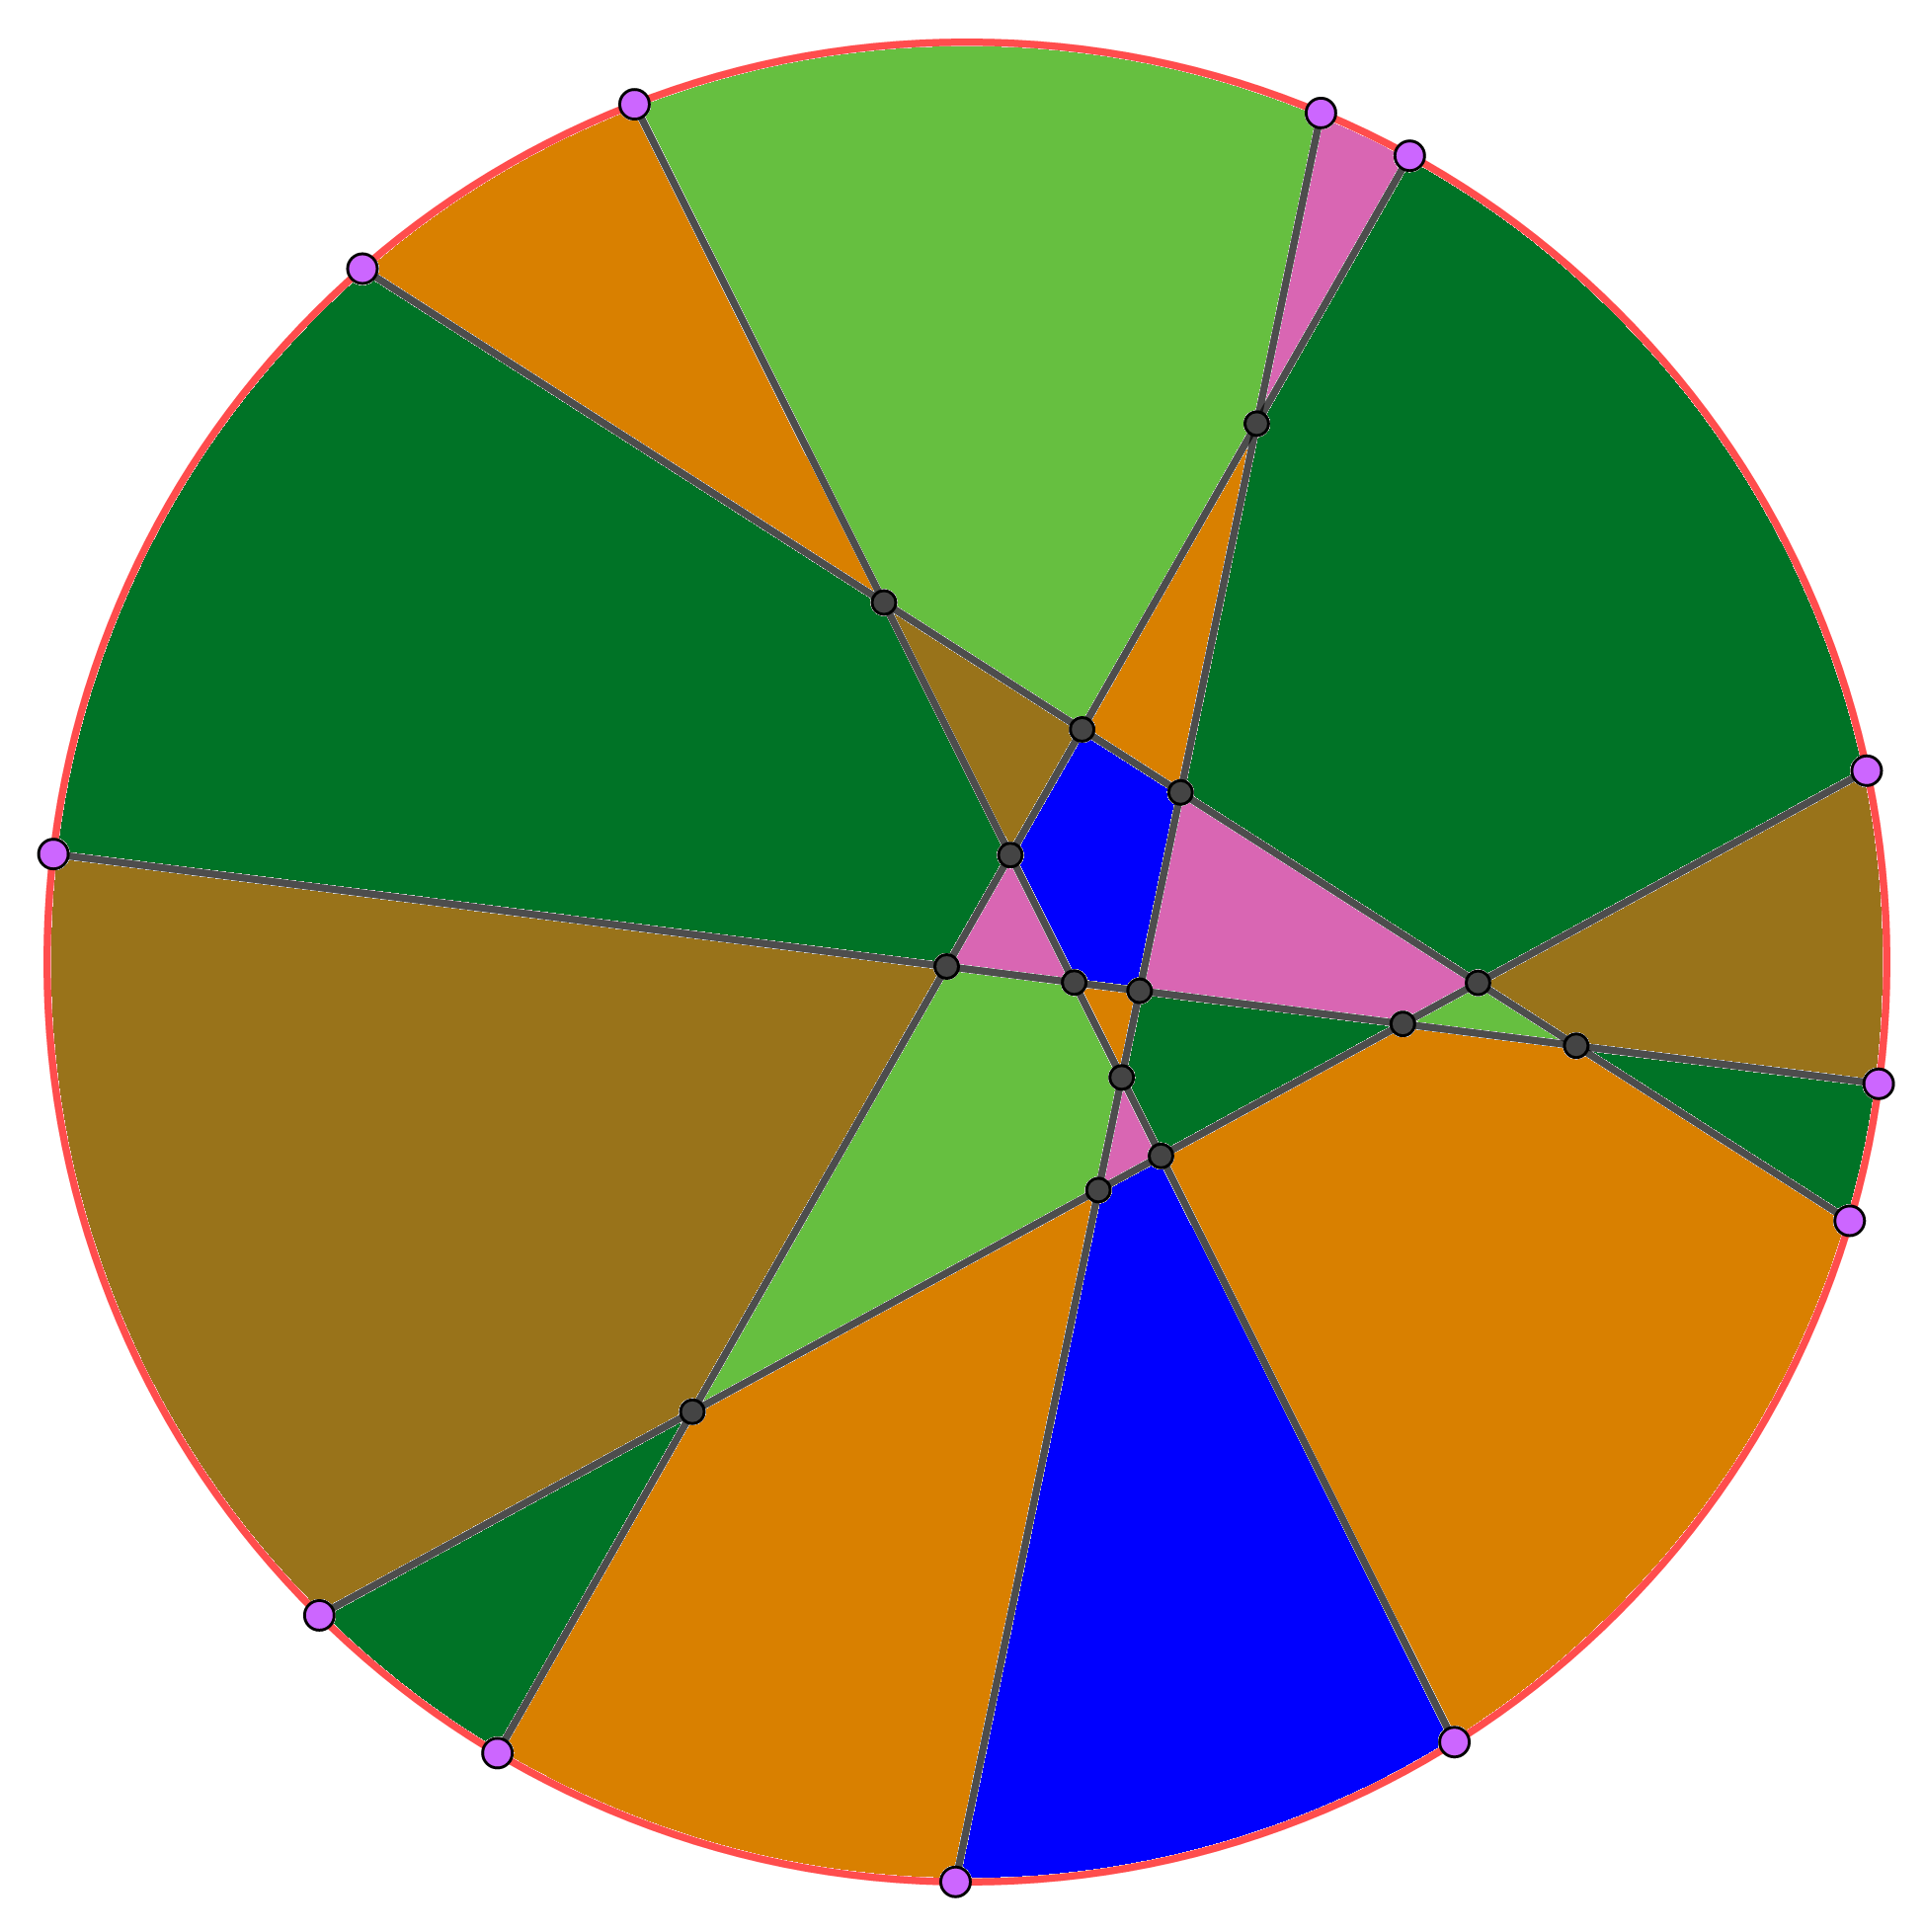
\includegraphics[width=\textwidth]{four_colour_1.png}
\caption{Figure 1}
\end{subfigure}
%
\begin{subfigure}[b]{0.45\textwidth}
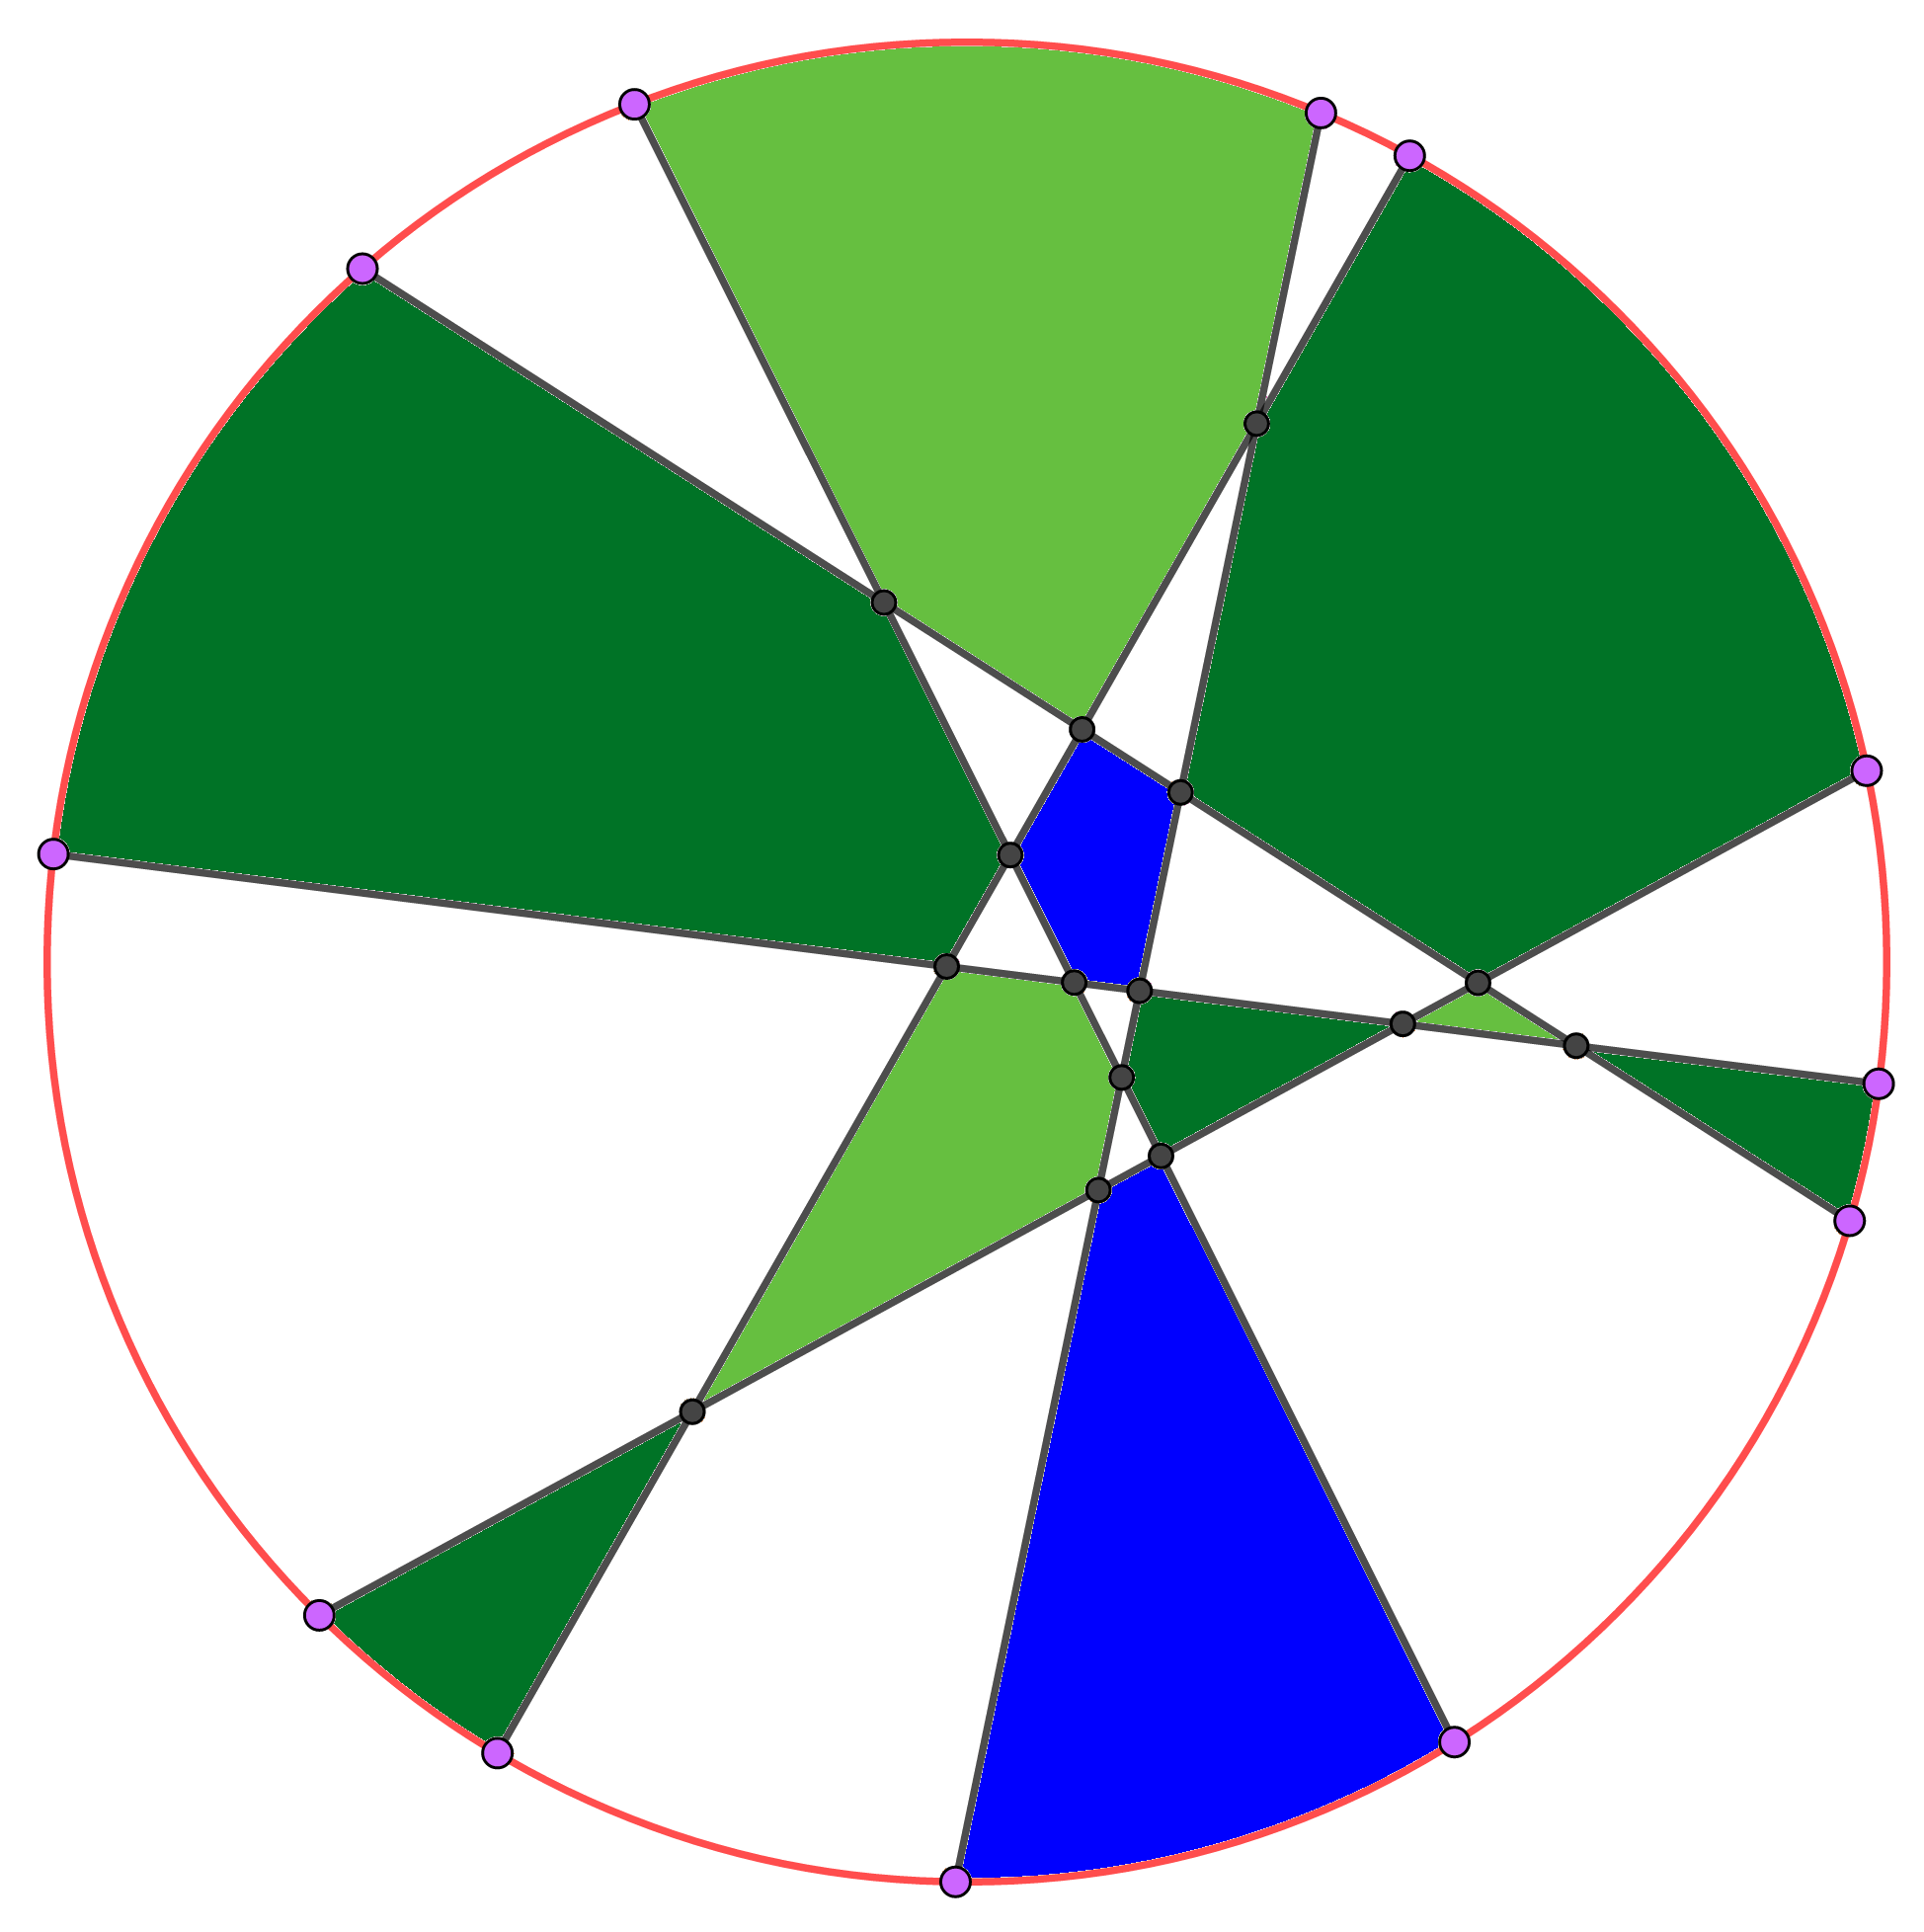
\includegraphics[width=\textwidth]{four_colour_2.png}
\caption{Figure 2}
\end{subfigure}

\begin{subfigure}[b]{0.45\textwidth} 
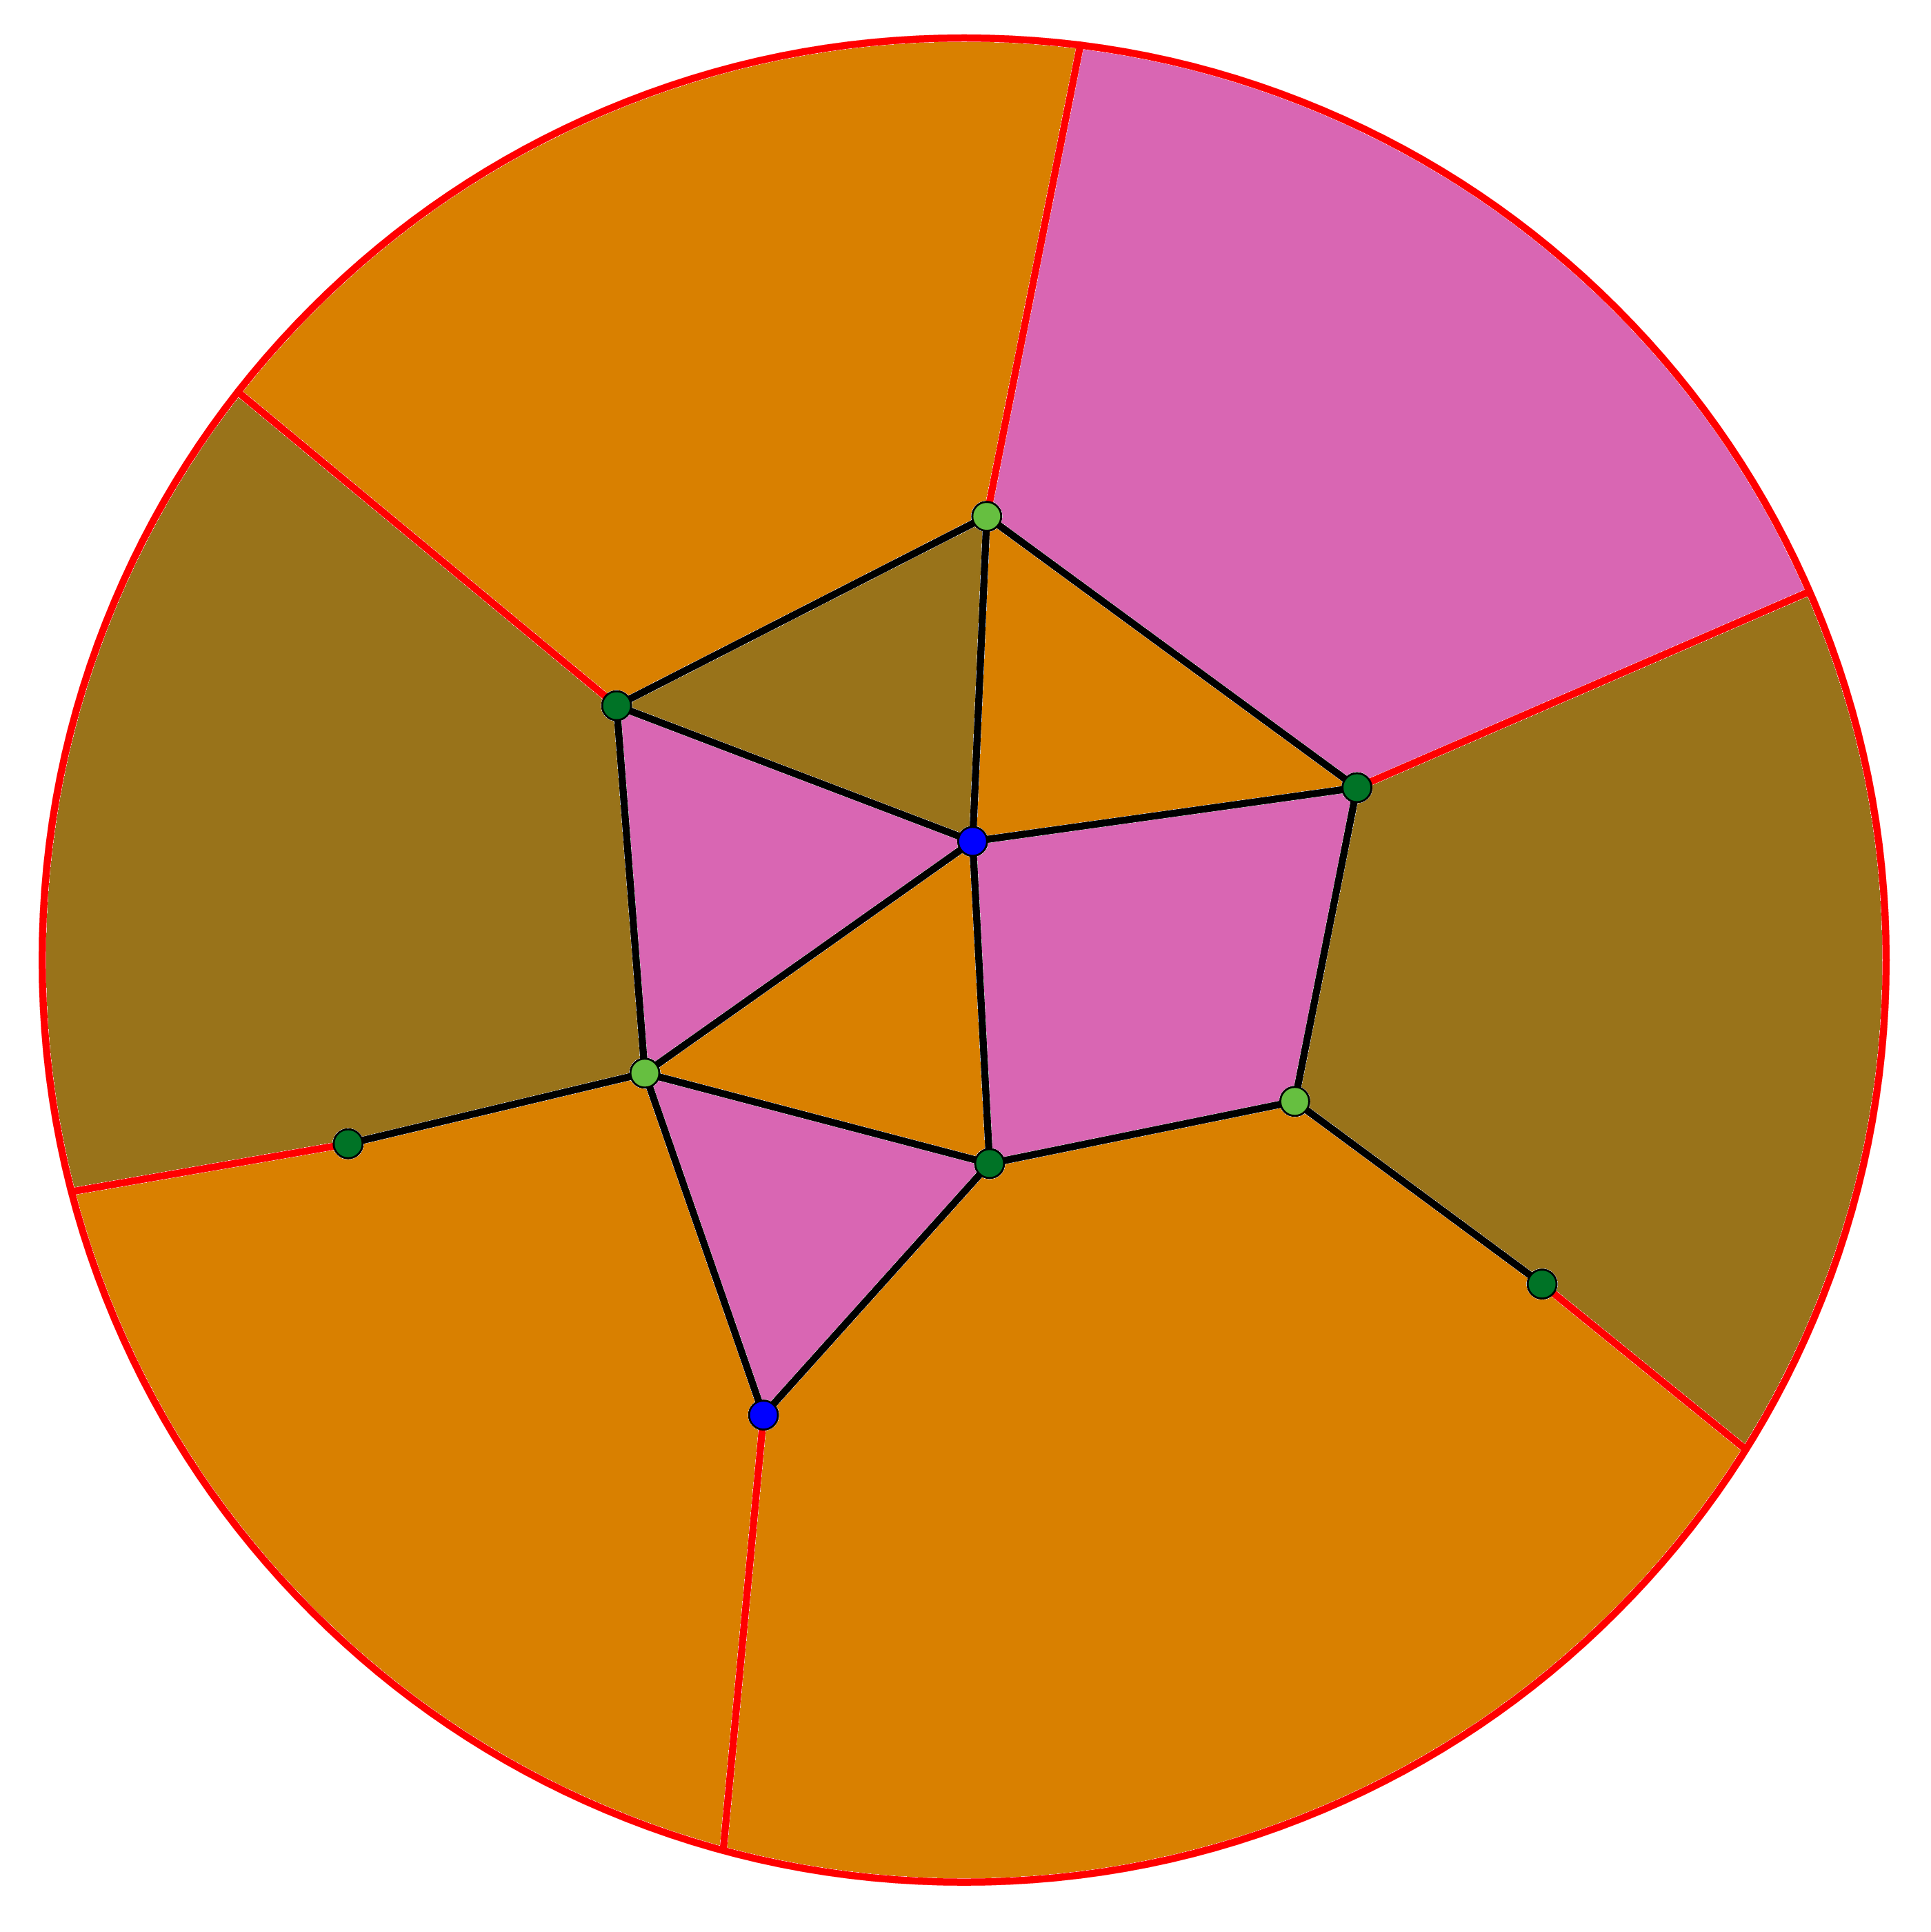
\includegraphics[width=\textwidth]{four_colour_3.png}
\caption{Figure 3}
\end{subfigure}
%
\begin{subfigure}[b]{0.45\textwidth}
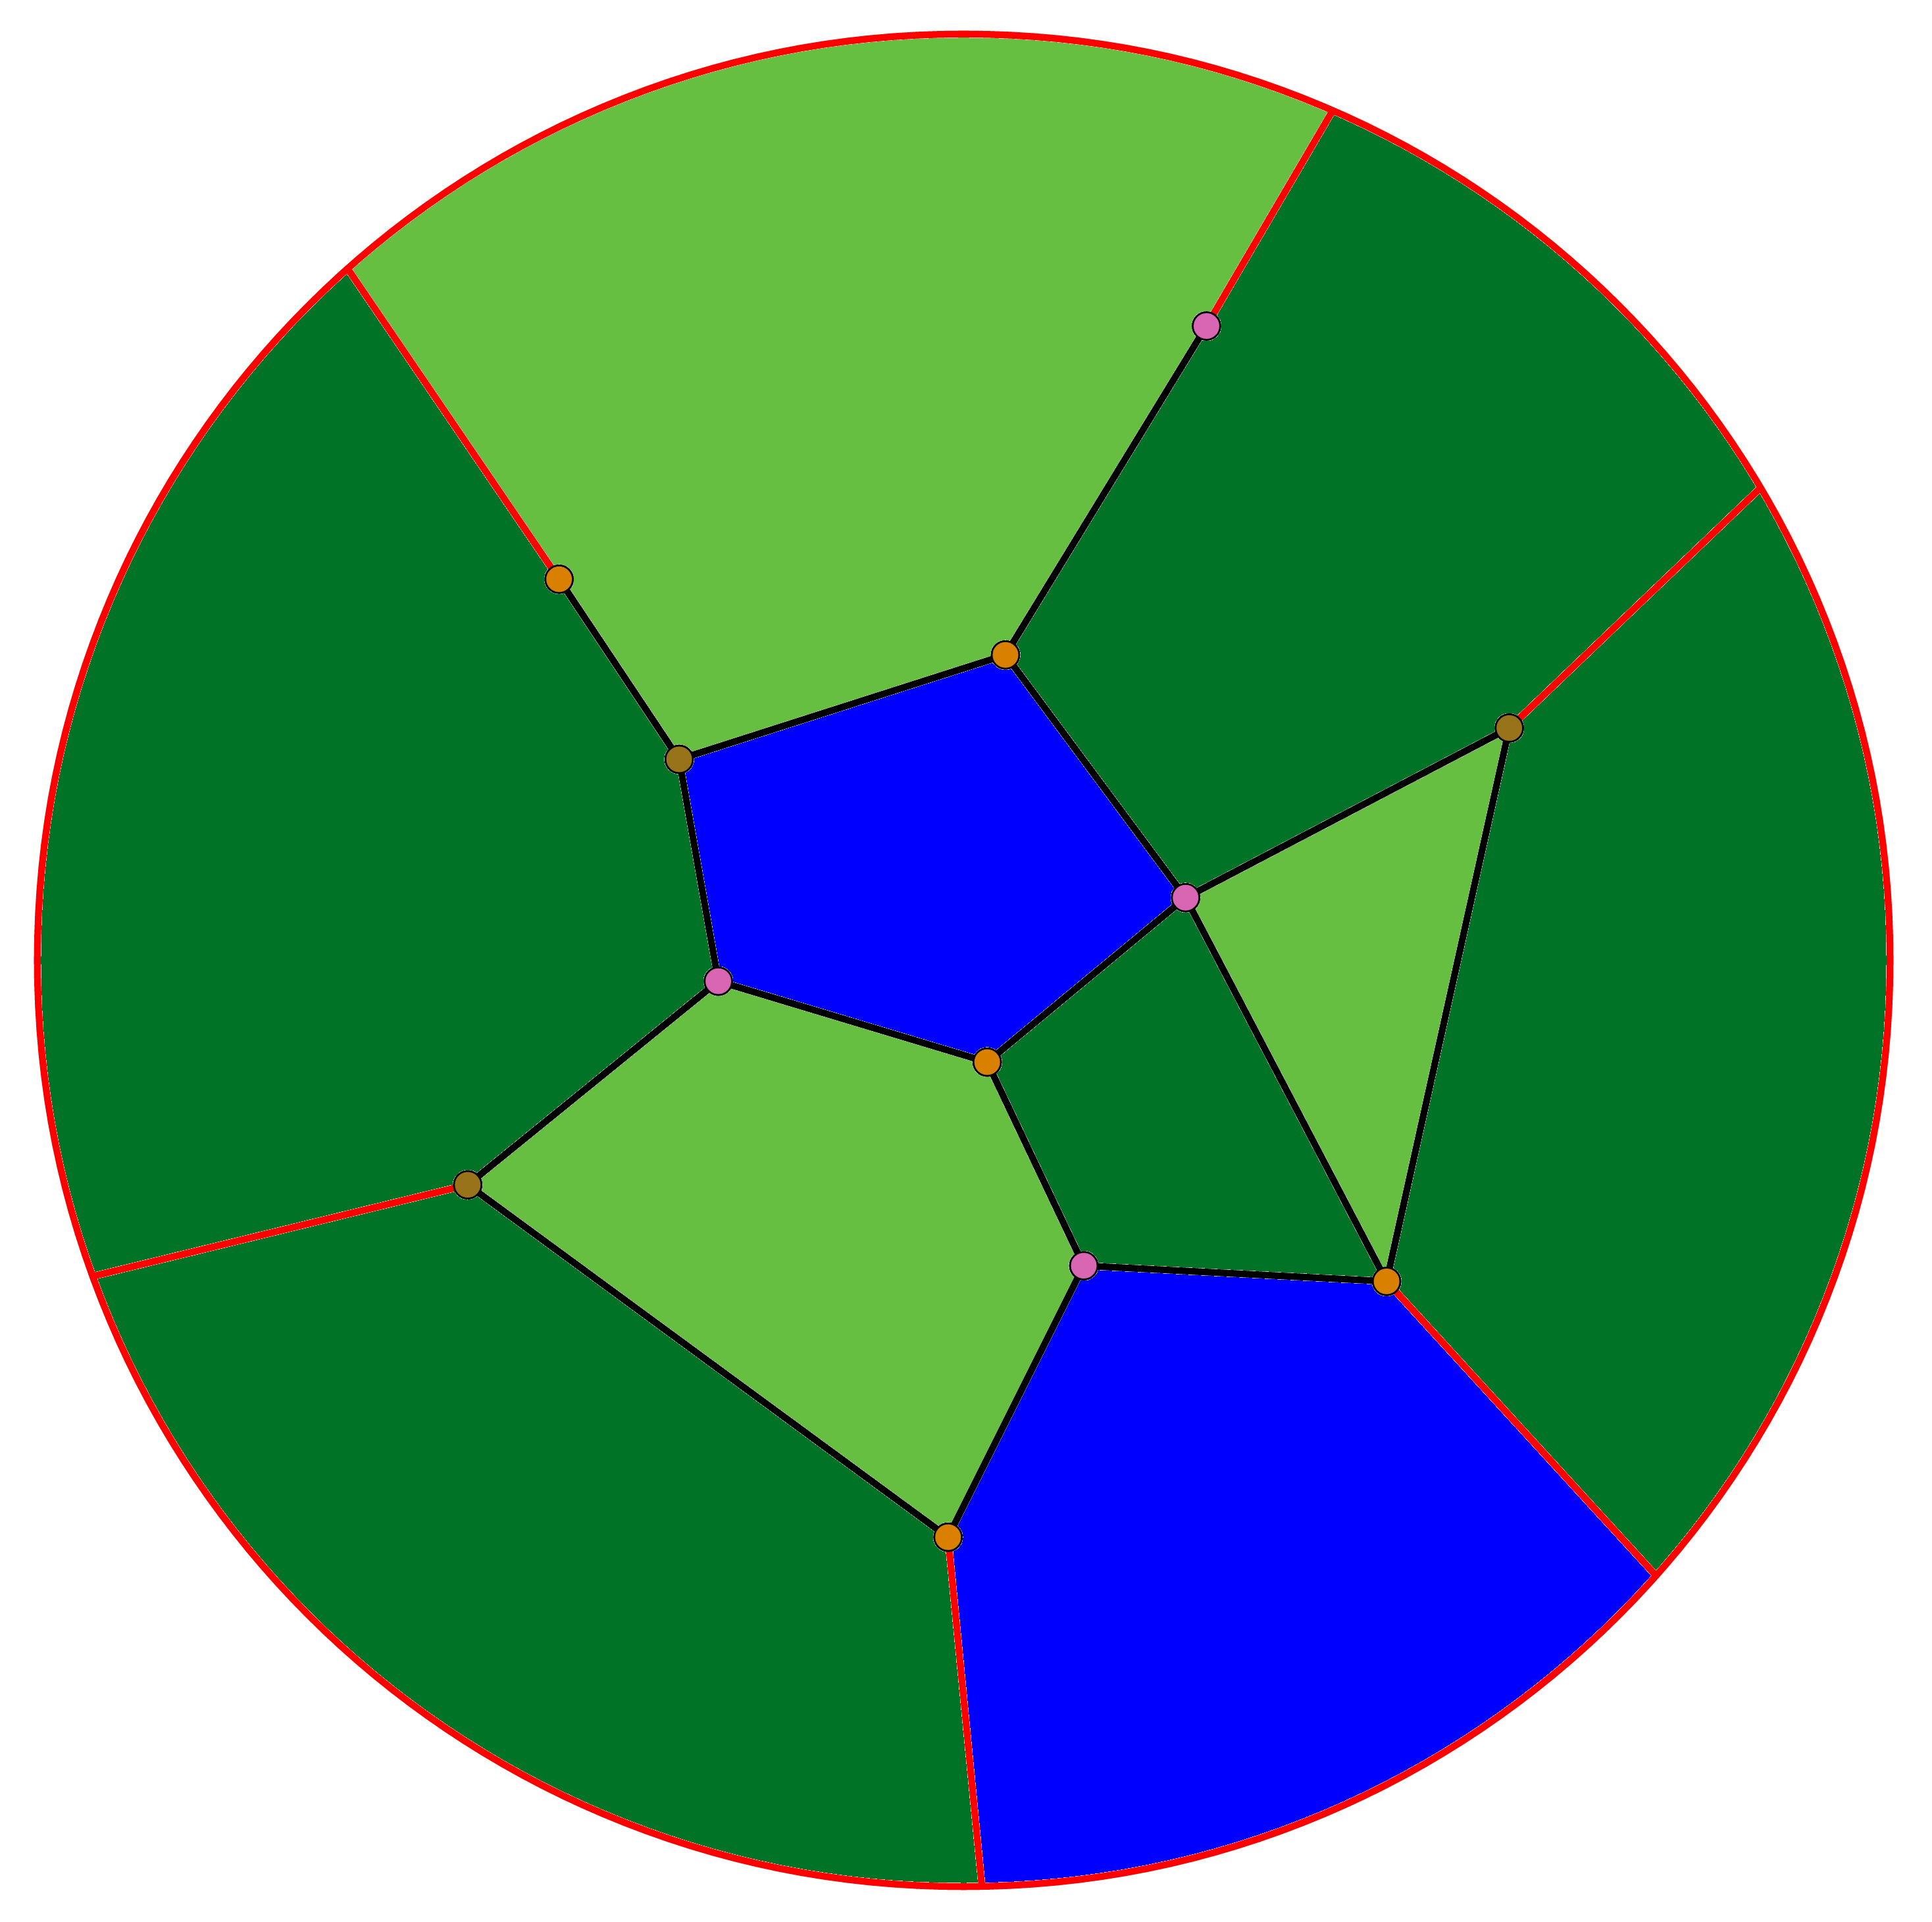
\includegraphics[width=\textwidth]{four_colour_4.png}
\caption{Figure 4}
\end{subfigure}

\caption{Problem~\ref{problem:four_colour}}
\end{figure}

Consider the $\binom{n}{2}$ points of intersections of the lines and draw a circle of colour red that contains all the intersection points (figure 1). Colour the lines black, colour the intersections black, and colour the intersections of the lines and the circle purple.

\textbf{Claim:} It is possible to colour the regions using two types of colours, say type red and type green, in such a way that no two regions of the same colour type have a common side.

\textbf{Proof of claim:} Consider a graph $G_0$ whose vertices are the regions and an edge corresponds to a common side. We shall show that $G_0$ is bipartite. It is enough to show that all cycles are of even length. Each walk from one vertex to another via an edge correspond to crossing one of the $n$ lines, but to get back to the starting point each line must be crossed an even number of times. Thus $G_0$ is bipartite and hence the vertices can be coloured with two types of colours (type blue and type red) in such a way that no two vertices of the same type share an edge.

Next we construct a graph $G_1$ (figure 3) whose vertices are the regions with type blue colour and draw an edge between two vertices of $G_1$ if the corresponding regions are in contact (via an intersection point in figure 1). Hence the edges of $G_1$ corresponds with the intersection points in figure 1. An extra vertex is added to $G_1$ to represent the red circle in figure 1 (this vertex is also represented by a red circle in figure 3) and edges from this vertex (depicted as red lines) are connected to vertices (regions) that touch the red line in figure 1.

Note that the faces of $G_1$ corresponds to the type red regions and the number of side of faces corresponds.

Construct $G_2$ similarly (figure 4) whose vertices are the regions with type red colour. Note that $G_1$ and $G_2$ are complements. And they are both planar and can both be coloured with four colours each by the \textbf{Four Colour Theorem}. So that's a total of $8$ colours.

Now if two regions share a common intersection pont then either they also share a side in which case they are of different colour type, or they are of same colour type (figure 2) and are adjacent in one of the graphs $G_1$ or $G_2$ and thus have different colour by the \textbf{Four Colour Theorem}.
}

\item\label{problem:sectors} A circle is divided into $n$ cells ($n \geq 3$). Each cell can be filled in with either $1$ or $0$. Choose any cell $\mathcal{C}$ occupied by $0$, change it into a $1$ and simultaneously change the symbols $x, y$ in the two adjacent cells to $\mathcal{C}$ to their complements $1 - x$, $1 - y$. We repeat this process as long as there exists a zero in some cell. In the initial configuration there is a $0$ in one cell and $1$s elsewhere. For which values of $n$ we can end this process?

\begin{figure}[!ht]
\centering
\includegraphics[width=0.6\textwidth]{Figure_1.mps}
\caption{Problem~\ref{problem:sectors}}
\end{figure}


\solution{%
First, remark that the process ends once we have $1$s in all cells. The answer to the question will depend on whether or not $n$ is divisible by $3$.

\begin{itemize}

\item If $3$ divides $n$, colour the cells successively white, red, black, white, red, black, etc\ldots Let $s_w, s_r, s_b$ be the sums of the numbers in white cells, red cells, and black cells, respectively. At each step of the process, the change is performed on one cell of every colour, so the sums $s_w, s_r, s_b$ change their parities simultaneously. Hence, if we start e.g.\ from $s_w = \frac{n}{3} - 1, s_r = \frac{n}{3}, s_b = \frac{n}{3}$, we will never arrive at $s_w = \frac{n}{3}, s_r = \frac{n}{3}, s_b = \frac{n}{3}$.

\item If $3$ does not divide $n$, it is possible to get ones everywhere using the following algorithm. Assume that at the start the only ``zero'' is in the third cell from the left, relative to an appropriate cyclic enumeration of cells. Thus the initial configuration is $110111 \dots 1111$. Consider the evolution
\begin{align*}
    110111 \dots 1111 \\
    101011 \dots 1111 \\
    100101 \dots 1111 \\
    100010 \dots 1111 \\
    \dots \dots \dots \dots \dots \\
    100000 \dots 0101 \\
    100000 \dots 0010 \\
    000000 \dots 0001
\end{align*}
(at each step we choose the rightmost ``zero'' and perform the allowed change, in that cell and in the neighbouring cells). In this way we obtain one $1$ and $n-1$ $0$s.

\begin{itemize}

\item If $n = 3k + 1$, then there are $3k$ zeros. Divide them into blocks of three and perform $k$ steps, in each step converting three successive zeros to ones, that clearly does the job.

\item If $n = 3k + 2$, we have $3k + 1$ zeros in the last configuration $000000 \dots 0001$. Changing the contents of the last three cells we reach that state $000000 \dots 0110$, with two ones and $3k$ zeros, and we may repeat the method of the previous case.

\end{itemize}

Thus is is possible to achieve the configuration with all ones if and only if $n$ is not divisible by $3$.

\end{itemize}
}

\end{enumerate}

\end{document}
